\documentclass[]{article}
\usepackage{lmodern}
\usepackage{amssymb,amsmath}
\usepackage{ifxetex,ifluatex}
\usepackage{fixltx2e} % provides \textsubscript
\ifnum 0\ifxetex 1\fi\ifluatex 1\fi=0 % if pdftex
  \usepackage[T1]{fontenc}
  \usepackage[utf8]{inputenc}
\else % if luatex or xelatex
  \ifxetex
    \usepackage{mathspec}
  \else
    \usepackage{fontspec}
  \fi
  \defaultfontfeatures{Ligatures=TeX,Scale=MatchLowercase}
\fi
% use upquote if available, for straight quotes in verbatim environments
\IfFileExists{upquote.sty}{\usepackage{upquote}}{}
% use microtype if available
\IfFileExists{microtype.sty}{%
\usepackage{microtype}
\UseMicrotypeSet[protrusion]{basicmath} % disable protrusion for tt fonts
}{}
\usepackage[margin=1in]{geometry}
\usepackage{hyperref}
\hypersetup{unicode=true,
            pdftitle={Teste T de Student para Duas Médias},
            pdfauthor={Douglas Vinícius},
            pdfborder={0 0 0},
            breaklinks=true}
\urlstyle{same}  % don't use monospace font for urls
\usepackage{graphicx,grffile}
\makeatletter
\def\maxwidth{\ifdim\Gin@nat@width>\linewidth\linewidth\else\Gin@nat@width\fi}
\def\maxheight{\ifdim\Gin@nat@height>\textheight\textheight\else\Gin@nat@height\fi}
\makeatother
% Scale images if necessary, so that they will not overflow the page
% margins by default, and it is still possible to overwrite the defaults
% using explicit options in \includegraphics[width, height, ...]{}
\setkeys{Gin}{width=\maxwidth,height=\maxheight,keepaspectratio}
\IfFileExists{parskip.sty}{%
\usepackage{parskip}
}{% else
\setlength{\parindent}{0pt}
\setlength{\parskip}{6pt plus 2pt minus 1pt}
}
\setlength{\emergencystretch}{3em}  % prevent overfull lines
\providecommand{\tightlist}{%
  \setlength{\itemsep}{0pt}\setlength{\parskip}{0pt}}
\setcounter{secnumdepth}{0}
% Redefines (sub)paragraphs to behave more like sections
\ifx\paragraph\undefined\else
\let\oldparagraph\paragraph
\renewcommand{\paragraph}[1]{\oldparagraph{#1}\mbox{}}
\fi
\ifx\subparagraph\undefined\else
\let\oldsubparagraph\subparagraph
\renewcommand{\subparagraph}[1]{\oldsubparagraph{#1}\mbox{}}
\fi

%%% Use protect on footnotes to avoid problems with footnotes in titles
\let\rmarkdownfootnote\footnote%
\def\footnote{\protect\rmarkdownfootnote}

%%% Change title format to be more compact
\usepackage{titling}

% Create subtitle command for use in maketitle
\providecommand{\subtitle}[1]{
  \posttitle{
    \begin{center}\large#1\end{center}
    }
}

\setlength{\droptitle}{-2em}

  \title{Teste T de Student para Duas Médias}
    \pretitle{\vspace{\droptitle}\centering\huge}
  \posttitle{\par}
    \author{Douglas Vinícius}
    \preauthor{\centering\large\emph}
  \postauthor{\par}
      \predate{\centering\large\emph}
  \postdate{\par}
    \date{2019-06-19}


\begin{document}
\maketitle

\href{pdf/slides2.pdf}{PDF} \href{slides/t-test.html}{Slides}

\begin{figure}
\centering
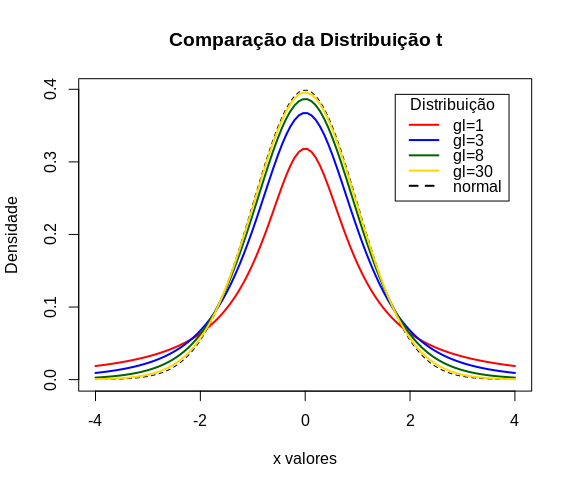
\includegraphics{img/Rplot1.png}
\caption{Distribuição t comparada com a normal.}
\end{figure}

Aplicação Shiny da distribuição t:
\href{https://douglas-vincius.shinyapps.io/T-test-shiny/}{T-test}

\hypertarget{teste-t-para-duas-mu-amostras-independentes-e-sigma-iguais}{%
\subsection{\texorpdfstring{Teste T para Duas \(\mu\) (Amostras
Independentes e \(\sigma²\)
Iguais)}{Teste T para Duas \textbackslash{}mu (Amostras Independentes e \textbackslash{}sigma² Iguais)}}\label{teste-t-para-duas-mu-amostras-independentes-e-sigma-iguais}}

Este método é usado para dados amostrais provenientes de duas amostras
independentes para o teste de hipóteses feitas sobre duas médias
populacionais. Destina a situação de dois desvios-padrão populacionais
são desconhecidos, mas se supõe que sejam iguais.

\hypertarget{requisitos}{%
\subsection{Requisitos}\label{requisitos}}

\begin{itemize}
\tightlist
\item
  Os dois desvios-padrão populacionais não são conhecidos, mas supõe-se
  quw sejam iguais, isto é, \(\sigma_{1}\) = \(\sigma_{2}\).
\item
  As duas amostras são independentes.
\item
  Ambas as amostras são \emph{amostras aleatórias simples}.
\item
  Uma ou as duas condições seguintes são satisfeitas: Os dois tamanhos
  amostrais são ambos \emph{grandes} (com n1 \textgreater{} 30 e n2
  \textgreater{} 30), ou ambas as amostras provêm de populações com
  distibuições normais. (Para pequenas amostras, a exigência de
  normalidade é relaxada, no sentido de que os procedimentos funcionam
  bem desde que não haja \emph{outliers} e os desvios da normalidade naõ
  sejam extremos.)
\end{itemize}

\hypertarget{o-que-e-amostras-independentes}{%
\subsubsection{O que é Amostras
Independentes?}\label{o-que-e-amostras-independentes}}

Duas amostras são \emph{independentes} se os valores amostrais de uma
população não estão relacionados ou, de alguma forma, emparelhados ou
combinados com os valores amostrais selecionados da outra população.

\hypertarget{estatistica-de-teste}{%
\subsubsection{Estatística de Teste:}\label{estatistica-de-teste}}

\[
t = \frac{(\bar{x}_1 - \bar{x}_2) - (\mu_1 - \mu_2)}{\sqrt{\frac{s_p²}{n_1} + \frac{s_p²}{n_2}}}
\] em que

\[
S_p² = \frac{(n_1 - 1)s_1² + (n_2 - 1)s_2²}{(n_1 - 1) + (n_2 - 1)}  \textrm{(Variância combinada)}
\] e o número de graus de liberdade é dado por gl \(= n_1 + n_2 - 2\).

\hypertarget{estimativa-de-intervalo-de-confianca-para-mu_1---mu_2}{%
\subsubsection{\texorpdfstring{Estimativa de intervalo de Confiança para
\(\mu_1 - \mu_2\)}{Estimativa de intervalo de Confiança para \textbackslash{}mu\_1 - \textbackslash{}mu\_2}}\label{estimativa-de-intervalo-de-confianca-para-mu_1---mu_2}}

\hypertarget{exemplo}{%
\subsubsection{Exemplo}\label{exemplo}}

\begin{itemize}
\tightlist
\item
  Um estudo objetivou analisar a associação entre a síndrome metabólica
  (SM) em indivíduos de origem japonesa, com mais de 30 anos de idade,
  residentes em um município do interior de São Paulo. -População 1:
  indivíduos com SM. -População 2: indivíduos sem SM.
\end{itemize}

Pergunta-se? Indivíduos com SM e sem SM possuem, em média, valores
iguais para a pressão arterial sistólica(PAS)?

\begin{itemize}
\tightlist
\item
  \(\mu_1\) é a média da PAS na população 1;
\item
  \(\mu_2\) é a média da PAS na população 2.
\end{itemize}

Testando as hipóteses: \[H_0: \mu_1 = \mu_2
\\H_a: \mu_1 \neq \mu_2\]

Lembrando que \(\sigma_1\) é o desvio padrão da PAS na população 1, e
\(\sigma_2\) é o desvio padrão da PAS na população 2; Pressupondo que
\[\sigma = \sigma_1 = \sigma_2\].

Teremos \[S_p² = \frac{(n_1 - 1)s_1² + (n_2 - 1)s_2²}{(n_1 + n_2 - 2)}\]

Lembrando que o teste tcal é um valor de uma variável aleatória que
segue uma distribuição t Student com n1 + n2 − 2 graus de liberdade.

\[t_{cal} = \frac{(\bar{x}_1 - \bar{x}_2)}{\sqrt{\frac{s_p²}{n_1} + \frac{s_p²}{n_2}}}\]
em que \[S_p² = \frac{(n_1 - 1)s_1² + (n_2 - 1)s_2²}{(n_1 + n_2 - 2)}\].

\begin{itemize}
\tightlist
\item
  Seja o tamanho das amostras da população 1 igual 52 e população 2
  igual 50.
\item
  Seja um nível de significância \(\alpha\) = 0,05; 1 - \(\alpha\) =
  0,95.
\item
  O número de graus de liberdade é 52+50-2=100.
\end{itemize}

Imagem adquirirda no
link:\url{https://douglas-vincius.shinyapps.io/T-test-shiny/}

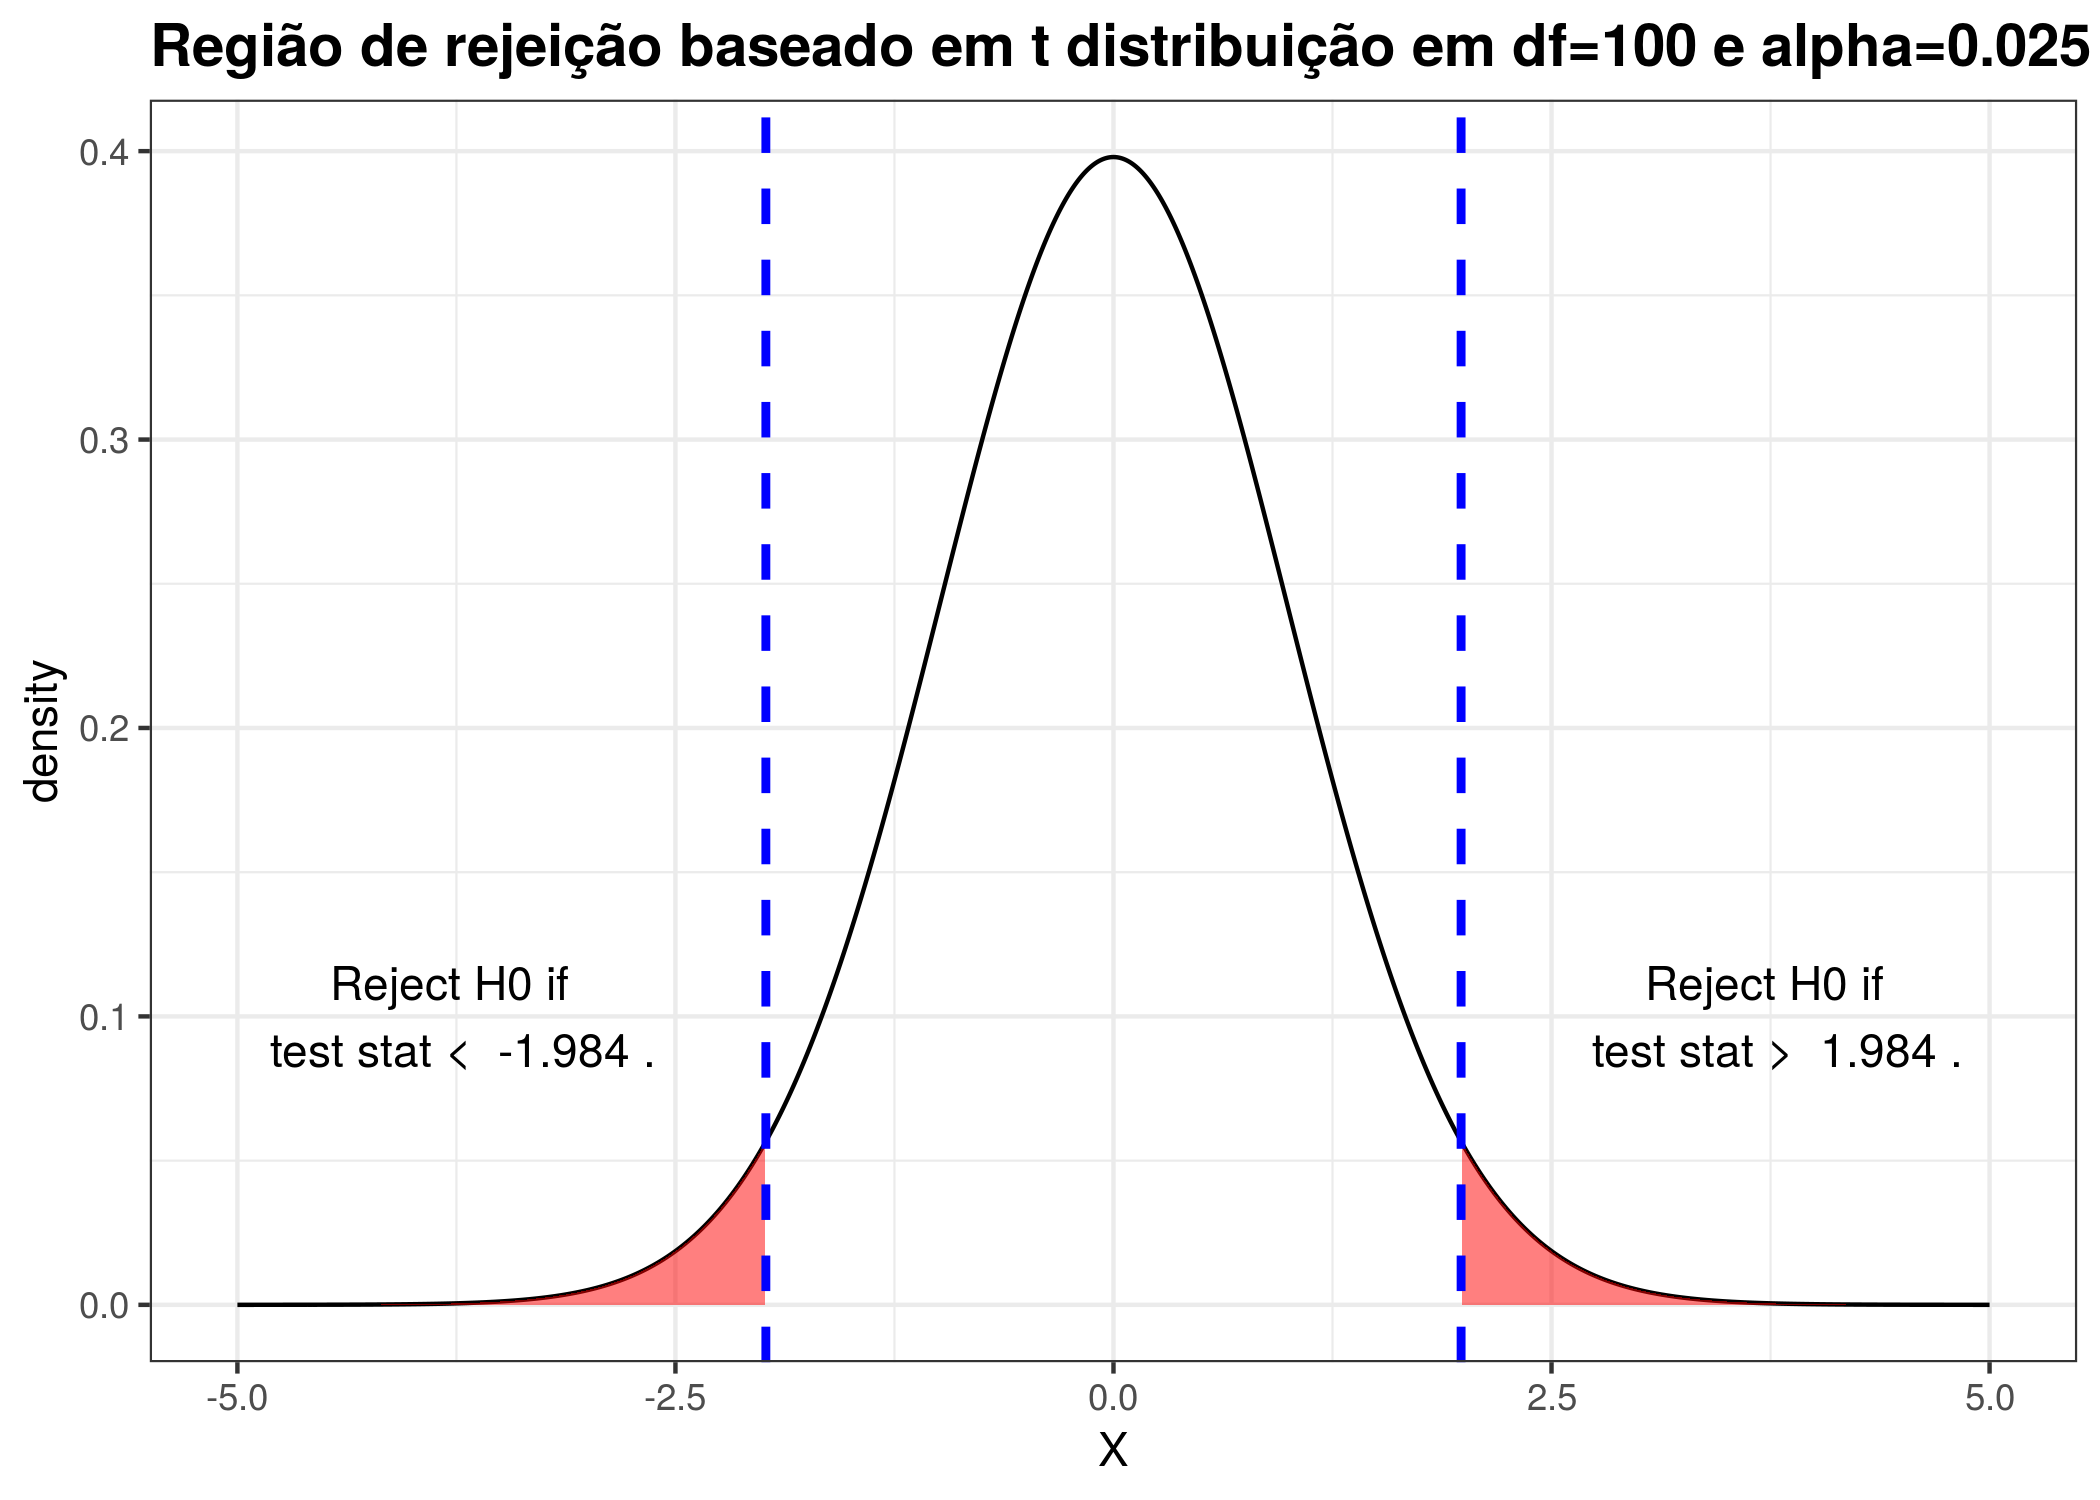
\includegraphics[width=565.44px,height=507.84px]{img/t_two_0.05}

-Não se rejeita H0 se encontrar um valor de tcal \textgreater{} -1,984 e
tcal \textless{} 1,984. \[
n_1 = 50 \ \ \ \ \ \ \ \ \ n_2 = 52
\\ \bar{x}_1 = 142,1\ \ mmHg \ \ \ \ \ \ \ \bar{x}_2 = 121,6\ \ mmHg
\\S_1 = 23\ \ mmHg \ \ \ \ \ \ \ S_2 = 21,3\ \ mmHg
\\\ 
\\S_p² = \frac{(50 - 1)23² + (52 - 1)21,3²}{(50 + 52 - 2)} = 492,0981
\\\
\\t_{cal} = \frac{(142,1 - 121,6)}{\sqrt{\frac{492,0981}{50} + \frac{492,0981}{52}}} \approx 4,67
\]

Como tcal \textgreater{} ttab, rejeita-se H0 para um nível de
significância de 0,05.

Assim temos evidências de que na população de indivíduos de origem
japonesa, com mais de 30 anos e residentes no município do interior de
São Paulo, com SM e sem SM possuem médias diferentes de PAS.


\end{document}
